\chapter{بهبود تشخیص اخبار جعلی با فراداده‌های حاصل از پردازش زبان}
\section{انگیزه}
در بسیاری از موارد  صحت‌سنجی یک خبر با استفاده از متن خبر کار بسیار دشوار و پیچیده‌ای است. اما بعضی‌از فراداده‌های مرتبط با اخبار می‌تواند در تشخیص موثق‌بودن این دسته از اخبار به ما کمک کند. در این فاز، به بررسی تأثیر استفاده از سه فراداده موضوع خبر، احساس خبر و موجودیت‌های نامدار موجود در خبر می‌پردازیم. با تحلیل و بررسی اخبار جعلی می‌توانیم دریابیم که آیا بعضی از موضوعات مثلاً سیاسی یا اجتماعی نسبت ‌به موضوعات دیگر مانند ورزشی بیشتر در معرض جعل خبر قرار دارد و خبر جعلی بیشتر در این موضوع مشخص تولید می‌شود یا خیر. دلیل این موضوع را می‌توان به‌دلیل تأثیرگذاری زیاد اخبار سیاسی و اجتماعی مطرح کرد. در صورت تأیید این فرضیه، انتظار می‌رود با دانستن موضوع هر خبر، بتوانیم درکنار متن خبر، با دقت بیشتری میزان جعلی‌بودن آن خبر را مشخص کنیم. علاوه بر این، یافتن موجودیت‌های نامدار و حس متن در هر خبر نیز می‌تواند اطلاعات نسبتاً مناسبی در مورد میزان صحت آن خبر ارائه دهد. در صورت تأیید این فرضیه نیز می‌توان حدس زد وجود اسامی خاص افراد، سازمان‌ها، مکان‌ها و ... در متن و یا حس مثبت یا منفی در متن می‌تواند به تشخیص جعلی‌بودن آن کمک کند. در ادامه این فصل به پردازش‌های متنی داده‌های خبری شامل دسته‌بندی موضوعی، تشخیص موجودیت‌های نامدار و تحلیل احساسات می‌پردازیم و در نهایت تأثیر آن‌ها را بررسی می‌نماییم.

\section{استخراج ویژگی‌های موضوعی مستندات}
یکی از ویژگی‌های مهم هر خبر، موضوع آن خبر است که کمک زیادی در تشخیص جعلی یا اصیل بودن آن‌ می‌کند. برای مثال، عمده اخبار جعلی در اخبار سیاسی است که با استفاده از ویژگی موضوع خبر می‌توانیم با دقت بیشتر جعلی‌بودن خبر را تشخیص دهیم. دو رویکرد برای بهره‌گیری از اطلاعات مربوط به موضوع اخبار فارسی در این پروژه مورد بررسی قرار گرفته است:
\begin{itemize}
	\item دسته‌بندی موضوعی با استفاده از روش‌های یادگیری با نظارت
	\item مدل‌سازی موضوعی با استفاده از روش‌های یادگیری بدون ‌نظارت
\end{itemize}

\subsection{دسته‌بندی بانظارت براساس 6 دسته مختلف}‌
موضوعات اخبار به دو صورت مشخص می‌شود. در یک حالت اخبار به صورت کلی به چند دسته اصلی تقسیم می‌شود و سپس در سطح دوم هر یک از این دسته‌ها به چند زیر دسته تقسیم می‌گردد. یکی از دسته‌بندی‌های استاندارد که در این زمینه وجود دارد، دسته‌بندی ارائه‌شده در پیکره همشهری است \citep{aleahmad2009hamshahri} که حاوی ۶ دسته کلی اخبار علمی و دانشگاهی، فرهنگی و هنری، سیاسی و اقتصادی، اجتماعی، بین‌المللی و ورزشی در این داده موجود است. برای دسته‌بندی اخبار بر اساس این ۶ دسته می‌توانیم از یک روش یادگیری بانظارت استفاده کنیم. همانند هر مسئله دسته‌بندی، مجموعه‌ای از اخبار شامل متن خبر و موضوع آن را به الگوریتم یادگیری می‌دهیم و پس از اتمام یادگیری، با استفاده از این مدل می‌توانیم موضوع اخبار جدید را تشخیص دهیم و از آن به‌عنوان ویژگی‌ای اضافه‌شده به بردار تعبیه متن خبر، استفاده کنیم. برای این منظور، در این پژوهش از دسته‌بندی با نظارت با استفاده از مدل ‌زبانی برت و برای آموزش مدل دسته‌بند از مجموعه اخبار همشهری که آمار آن در \tablename~\ref{table.hamshahri} آمده، ‌استفاده کرده‌ایم.
پس‌ از آموزش دسته‌بند، عملیات دسته‌بندی می‌تواند بر روی هر خبری انجام شود و حاصل این دسته‌بندی به‌صورت یک بردار تک‌روشنِ شش‌بُعدی نمایش داده شود تا از آن به‌عنوان ویژگی در آموزش مدل‌های تشخیص اخبار جعلی بهره برده شود.

\begin{table} [h!]
	\caption{آمار و اطلاعات مربوط به دادگان همشهری}
	\label{table.hamshahri}
	\begin{center}
		\begin{tabular}{|M{6cm}|M{4cm}|}
			\hline
			ویژگی & مقدار \\
			\hline
			\hline
			حجم دادگان & 564 مگابایت \\ \hline
			نوع اسناد & متن \\ \hline
			تعداد اسناد & $166,774$ \\ \hline
			تعداد واژه‌های یکتا & $417,339$ \\ \hline
			میانگین طول سند & 380 واژه \\ \hline
			تعداد دسته‌ها & 82 \\ \hline
			تعداد موضوعات & 65 \\ \hline
		\end{tabular}
	\end{center}
\end{table}

\subsection{دسته‌بندی بدون‌ نظارت براساس روش تخصیص نهان دیریکله}
\label{section.lda_classification}
همانطور که پیش‌تر در بخش \ref{sec:lda} اشاره شد، روش تخصیص نهان دیریکله \citep{blei2003latent} یک روش بدون‌ نظارت بر مبنای مدل‌های احتمالاتی است که در آن با دریافت  پیکره  اخبار، دسته‌های موضوعات مستندات را انتخاب می‌کند. هر دسته باتوجه ‌به هم‌نشینی واژه‌ها در پیکره متن مشخص می‌شود. بنابراین نماینده هر موضوع مجموعه‌ای از واژه‌ها خواهد بود که باید برچسب آن‌ها مشخص گردد. این روش  ۲ ماتریس خروجی تولید می‌کند:
\begin{itemize}
	\item
	ماتریس واژه-موضوع، که نشان می‌دهد در هر موضوع استنتاج‌شده چه واژه‌هایی قرار دارد.
	\item
	ماتریس سند-موضوع، که نشان‌دهنده آن است که هر سند چه سهمی از موضوعات مختلف را دارد. بیشترین سهم نشان‌دهنده موضوع اصلی آن سند خواهد بود.
\end{itemize}
یکی از چالش‌های اصلی این روش پیداکردن مقدار بهینه برای تعداد موضوعات است؛ چراکه اگر این مقدار خیلی زیاد شود، موضوعات نسبتاً مرتبط از یکدیگر جدا خواهند شد و خطای احتمالی برای پیش‌بینی یک خبر جدید بیشتر می‌شود. از طرف دیگر، اگر تعداد موضوعات خیلی کم انتخاب شود، موضوعات نامرتبط دارای یک برچسب موضوعی یکسان خواهد شد. یکی از راه‌های پیداکردن مقدار بهینه برای موضوعات اخبار درکنارِ داشتنِ آگاهی از مقدار حدودی تعداد موضوعات معمول در خبرگزاری‌ها، استفاده از تعدادی است که خطای کلی مدل به کمترین مقدار برسد. برای این منظور، چند عدد متفاوت برای مدل‌سازی موضوعی انتخاب خواهد شد و با بررسی خروجی مدل و ارزیابی کیفی، به‌صورت تجربی تعداد بهینه موضوعات مشخص می‌گردد.


\section{تشخیص موجودیت‌های نامدار}
یکی از عملیات‌های پایه در پردازش‌ زبان طبیعی شناسایی موجودیت­‌های نامدار است که در آن تمامی­ اسامی خاص موجود در متن استخراج می‌گردد و به گروه‌های ازپیش ‌تعریف‌شده‌ای مانند اسم افراد، سازمان‌ها، مکان‌ها و ... دسته‌بندی می‌شود. شناسایی موجودیت­‌های نامدار در بسیاری از عملیات‌ها مانند جستجوهای معنادار\LTRfootnote{Semantic Search}، ترجمه ماشینی\LTRfootnote{Machine Translation}، استخراج اطلاعات از متن\LTRfootnote{Information Extraction}، مرجع‌یابی در متن\LTRfootnote{Co-reference Resolution}، سیستم­‌های پرسش و پاسخ\LTRfootnote{Question Answering Systems} ، سیستم‌های خبره\LTRfootnote{Expert Systems} ، کشف دانش\LTRfootnote{Knowledge Discovery} ، مدیریت دانش\LTRfootnote{Knowledge Management}، تحلیل احساسات\LTRfootnote{Sentiment Analysis}، بازیابی اطلاعات\LTRfootnote{Information Retrieval}، تحلیل خبر\LTRfootnote{News Analysis} و بسیاری دیگر از شاخه های مرتبط با پردازش زبان­ طبیعی کاربرد دارد. 
به منظور استخراج موجودیت‌های نامدار دو روش قاعده‌مند و آماری وجود دارد \citep{Jurafsky2009}. در روش‌­های قاعده‌مند، براساس قوانین از‌پیش مشخص‌شده موجودیت‌­های نامدار تشخیص داده می‌­شوند. در روش آماری، از با استفاده از مفاهیم یادگیری ماشین به دسته­‌بندی موجودیت­‌های نامدار پرداخته می‌شود. در روش دسته‌بندی بانظارت، از پیکره‌هایی که موجودیت‌های نامدار مشخص دارند استفاده می‌شود و مدل یاد می‌گیرد تا چگونه دسته‌بندی موجودیت‌های نامدار جدید را انجام دهد.
موجودیت‌های نامدار می‌توانند نقش مهمی را در تشخیص اخبار جعلی ایفا کنند چراکه اخبار جعلی توزیع متفاوتی از اسامی خاص مانند افراد را نسبت به اخبار اصیل می‌توانند داشته باشند. در این پروژه ما از یک مدل آموزش دیده که به صورت بانظارت آموزش داده شده است، استفاده کردیم.

\cite{Thesis_abdolah}
با استفاده از مدل ایکس.ال.ام-روبرتا به نتایج قابل‌قبولی در تشخیص موجودیت‌های نامدار رسیده است و ما برای استخراج موجودیت‌های نامدار هر خبر از این مدل استفاده می‌کنیم. مسئله پر اهمیت در آموزش مدل، داده‌های یادگیری هستند. بسیاری از پیکره‌های معرفی شده در زبان فارسی تنها موجودیت‌های نامدار مربوط به نام اشخاص، موقعیت‌های مکانی و اسامی سازمان‌ها را شامل می‌شوند. به منظور استخراج موجودیت‌های بیشتر در متن ورودی، برای آموزش این مدل از پیکره موجودیت‌های نامدار تهیه‌شده در آزمایشگاه پردازش زبان طبیعی دانشگاه صنعتی امیرکبیر که شامل ۱۵ موجودیت نامدار است، استفاده شده است \citep{momtazi2020named}.
این دادگان شامل ۳۱ برچسب برای مشخص کردن ۱۵ نوع موجودیت متفاوت است که شامل اسم شخص مفرد، اسم شخص جمع، موقعیت مکانی، اسم سازمان، زبان، ملیت، رخداد، شغل، کتاب، اسم فیلم، تاریخ، مذهب، عنوان علمی و دانش، روزنامه و سایر اسامی خاص ذکرنشده در زبان فارسی می‌باشد. جدول \ref{table.NER_tags} به تفضیل به شرح و بررسی برچسب­‌های استفاده‌شده برای دادگان می‌پردازد.

\begin{table}
	\caption{راهنمای برچسب واژگان}
	\label{table.NER_tags}
	\begin{center}
		\small
		\begin{tabular}{|P{1.2cm}|P{2cm}|P{2cm}|P{8cm}|}
			\hline
			برچسب & تعریف انگلیسی برچسب & تعریف فارسی برچسب & توضیحات \\
			\hline
			\lr{O} & \lr{Out} &
			هیچ & واژه مورد نظر از موجودیت‌های نامدار نیست. \\
			\hline
			\lr{PEI} & \lr{Person Individual} &
			شخص مفرد & این علامت به نام شخص اشاره دارد. \\
			\hline
			\lr{PEG} & \lr{Person Group} &
			اسم خاص گروه & این علامت به موجودیت نامداری اشاره دارد که به‌صورت جمع آمده‌است.\\
			\hline
			\lr{LOC} & \lr{Location} &
			موقعیت مکانی & واژه مورد نظر این برچسب به موقعیت مکانی خاصی اشاره دارد. \\
			\hline
			\lr{ORG} & \lr{Organization} &
			سازمان  & اسامی سازمان‌­ها و مؤسسات مختلف با این برچسب نشان داده می‌­شود. \\
			\hline
			\lr{LAN} & \lr{Language} &
			زبان & این برچسب نشان‌دهنده زبان‌­های مختلف است. \\
			\hline
			\lr{NAT} & \lr{Nationality} &
			ملیت & ملیت­‌های مختلف با این علامت تعیین می‌­شود. \\
			\hline
			\lr{EVN} & \lr{Events} &
			رخدادها & رخدادها و وقایع خاص را با این برچسب نشان دادیم. \\
			\hline
			\lr{JOB} & \lr{Job} &
			شغل & این برچسب نمایانگر مشاغل است. \\
			\hline
			\lr{BOK} & \lr{Book} &
			کتاب & اسامی کتاب‌­ها با این برچسب مشخص می‌شود. \\
			\hline
			\lr{FLM} & \lr{Film} &
			فیلم & نام فیلم‌­های مختلف با این برچسب تعیین می‌­شود. \\
			\hline
			\lr{DTE} & \lr{Date} &
			تاریخ & برای نشان‌دادن تاریخ و دوره‌های مختلف از برچسب استفاده شده‌است. \\
			\hline
			\lr{REL} & \lr{Religion} &
			مذهب & این برچسب تعیین‌کننده مذاهب مختلف است. \\
			\hline
			\lr{FLD} & \lr{Field} &
			زمینه & زمینه‌ها و دانش‌­های مختلف با این برچسب تعیین گردیده‌است. \\
			\hline
			\lr{MAG} & \lr{Magazine} &
			روزنامه و مجله & اسامی روزنامه‌ها و مجلات با این برچسب آمده‌است. \\
			\hline
			\lr{OTH} & \lr{Other} &
			سایرین & اگر واژه‌ای به‌عنوان موجودیت نامدار باشد ولی در بین موجودیت­‌های معرفی‌شده در بالا نباشد با این برچسب مشخص می‌­شود. \\
			\hline
			
		\end{tabular}
	\end{center}
\end{table}


\section{تحلیل احساسات}
نظرکاوی یا تحلیل احساسات، مطالعه محاسباتی نظرات کاربران حول محصولات، خدمات، سازمان‌ها، اشخاص، رویدادها و جنبه‌های مختلف آن است. در سال‌های اخیر این حوزه یکی از حوزه‌های پژوهشی فعال در پردازش زبان‌های طبیعی بوده است. نظرکاوی در سطوح مختلف سند، جمله و جنبه مورد مطالعه قرار گرفته‌است. در حوزه کالا و خدمات هنگام تصمیم‌گیری عقاید دیگران تأثیر به‌سزایی در تصمیم نهایی دارد. در دنیای واقعی، شرکت‌ها همواره نیازمند عقاید مردم برای بهبود کیفیت و توسعه خدمات خود است. در دنیای نشر خبر، سوگیری احساسی اخبار یکی از جنبه‌های مؤثر در تحلیل خبر می‌باشد. مثبت یا منفی بودن یک خبر می‌تواند جنبه‌های مختلفی از تحلیل آن خبر را فراهم آورد. درحال‌حاضر داده‌های متنی  بخش عظیمی از شبکه‌های اجتماعی، فروشگاهای اینترنتی و انواع مختلف سامانه‌های ارتباطی را در بر گرفته‌است. از این داده‌ها می‌توان در راستای درک احساسات کاربران به مطالب مختلف مانند یک محصول، یک نوشته موضوعی و ... استفاده کرد. 

نظر‌کاوی در سال 2002 توسط \citet{pang2002} معرفی شد. با روی‌کارآمدن شبکه‌های اجتماعی و تأثیر روزافزون آن‌ها بر زندگی مردم، اهمیت نظر‌کاوی و کاربردهای آن بیشتر مشخص گردید. باتوجه‌به این که افراد با حضور در این شبکه‌ها به بیان نظرات، عقاید و دیدگاه‌های خود درباره کلیه مسائل سیاسی، اجتماعی، فرهنگی، اقتصادی و حتی فردی می‌پردازد، تحلیل احساسات بیشتر از هر چیز در شبکه‌های اجتماعی مورد توجه قرار گرفته‌است. در کنار بستری که در شبکه‌های اجتماعی فراهم شده‌است، متون موجود در داده‌های خبری نیز می‌توانند دارای حس مثبت یا منفی باشد که به تحلیل آن کمک می‌نماید.

برای استفاده از تحلیل احساسات در تشخیص اخبار جعلی، تحلیل احساس در سطح سند مورد توجه این پژوهش قرار گرفته‌است و با بهره‌گیری از یک مدل مبتنی‌ بر یادگیری عمیق حس موجود در متن به‌صورت یک بردار دو بعدی برای حس مثبت و منفی مشخص می‌گردد. خروجی این مدل به‌عنوان یکی از ویژگی‌های ورودی در مدل تشخیص اخبار جعلی استفاده خواهد شد.

برای پیاده‌سازی بخش تشخیص احساسات از شبکه پیچشی استفاده شده‌است. باتوجه‌ به این که پایه اصلی تحلیل احساسات دسته‌بندی متون است، ساختار شبکه پیچشی مورد استفاده در این بخش مشابه شبکه پیچشی‌ای است که در تشخیص خبر جعلی مورد استفاده قرار گرفته‌ است و توضیحات آن در بخش \ref{sec:bert_cnn} آمده ‌است.  بازنمایی مورد استفاده در این شبکه نیز بازنمایی ایکس.ال.ام-روبرتا می‌باشد.

\section{نتایج حاصل از استفاده از پردازش‌های متنی در تشخیص اخبار}
در فصل گذشته، با بررسی و مقایسه مدل‌های از پیش آموزش دیده، بهترین مدل بازنمایی اخبار ورودی را انتخاب کردیم. در این بخش می‌خواهیم با استفاده از هر دو مدل دسته‌بند شبکه پیشرو پرسپترون و شبکه عصبی پیچشی و استفاده از مدل پارس‌برت برای بازنمایی اخبار، از فراداده‌هایی مانند موضوع خبر، موجودیت‌های نامدار و یا حس متن در کنار بردار بازنمایی متن خبر استفاده کنیم.

برای استفاده از ویژگی موضوع خبر در رویکرد اول  یک بردار ویژگی ۶ بعدی حاصل از دسته‌بندی موضوعی اخبار و در رویکرد دوم یک بردار ویژگی ۵۰ بعدی حاصل از تخصیص نهان دیریکله خواهیم داشت. بازنمایی خروجی تحلیل احساس نیز یک بردار دو بعدی است که هر درایه آن نشان‌دهنده مثبت و یا منفی بودن آن خبر است. همچنین، اطلاعات مربوط به موجودیت‌های نامدار موجود در یک خبر با استفاده از یک بردار شامل ۱۵ ویژگی بازنمایی می‌شود. برای نمونه،  در جدول \ref{table.ner_example} نمونه‌ای از یک جمله برچسب‌گذاری‌شده نمایش داده شده‌است. در بردار ۱۵تایی حاصل از این جمله، درایه مربوط به موجودیت کتاب مقدار ۲، درایه‌های مربوط به موجودیت‌های زبان، شخص مفرد، شغل و تاریخ مقدار ۱ و سایر درایه‌ها مقدار صفر خواهد داشت. 
\begin{table}[h!]
	\caption{مثال از یک جمله برچسب‌خورده توسط مدل تشخیص موجودیت نامدار}
	\label{table.ner_example}
	\begin{center}
		\begin{tabular}{|c|c|}
			\hline
			واژه & برچسب \\
			\hline
			\hline
			کتاب &\lr{b-BOK} \\
			گلستان & \lr{i-BOK} \\
			و & \lr{O} \\
			کتاب & \lr{b-BOK} \\
			بوستان & \lr{i-BOK} \\
			از & \lr{O} \\
			شاهکارهای & \lr{O} \\
			ادب & \lr{O} \\
			فارسی & \lr{b-LAN} \\
			و & \lr{O} \\
			اثر & \lr{O} \\
			سعدی & \lr{b-PEI} \\
			شاعر & \lr{b-JOB} \\
			قرن & \lr{b-DTE} \\
			ششم & \lr{i-DTE} \\
			هجری & \lr{i-DTE} \\
			است & \lr{O} \\
			\hline
			
		\end{tabular}
	\end{center}
\end{table}


به‌منظور استفاده از ویژگی‌های فراداده‌های مختلف،  بردار‌های این ویژگی‌ها را ابتدا به یک لایه چگال با همان تعداد نورون وارد می‌کنیم و پس‌از‌ آن بردار خروجی لایه چگال را به انتهای بردار ویژگی‌های نهایی استخراج‌شده از متن اخبار الحاق می‌کنیم. درنهایت پس‌ از ساخت بردار ویژگی جدید، شامل ویژگی‌های متن و فراداده‌ها، آن را وارد یک لایه پرسپترون می‌کنیم تا برچسب اخبار مشخص شود. شِمای کلی مدل ارائه‌شده برای استفاده از تمام فراداده‌ها در کنار ویژگی‌های مبتنی بر بافت اخبار در شکل \ref{fig.all_features} ارائه شده است.

\begin{figure}[!t]
	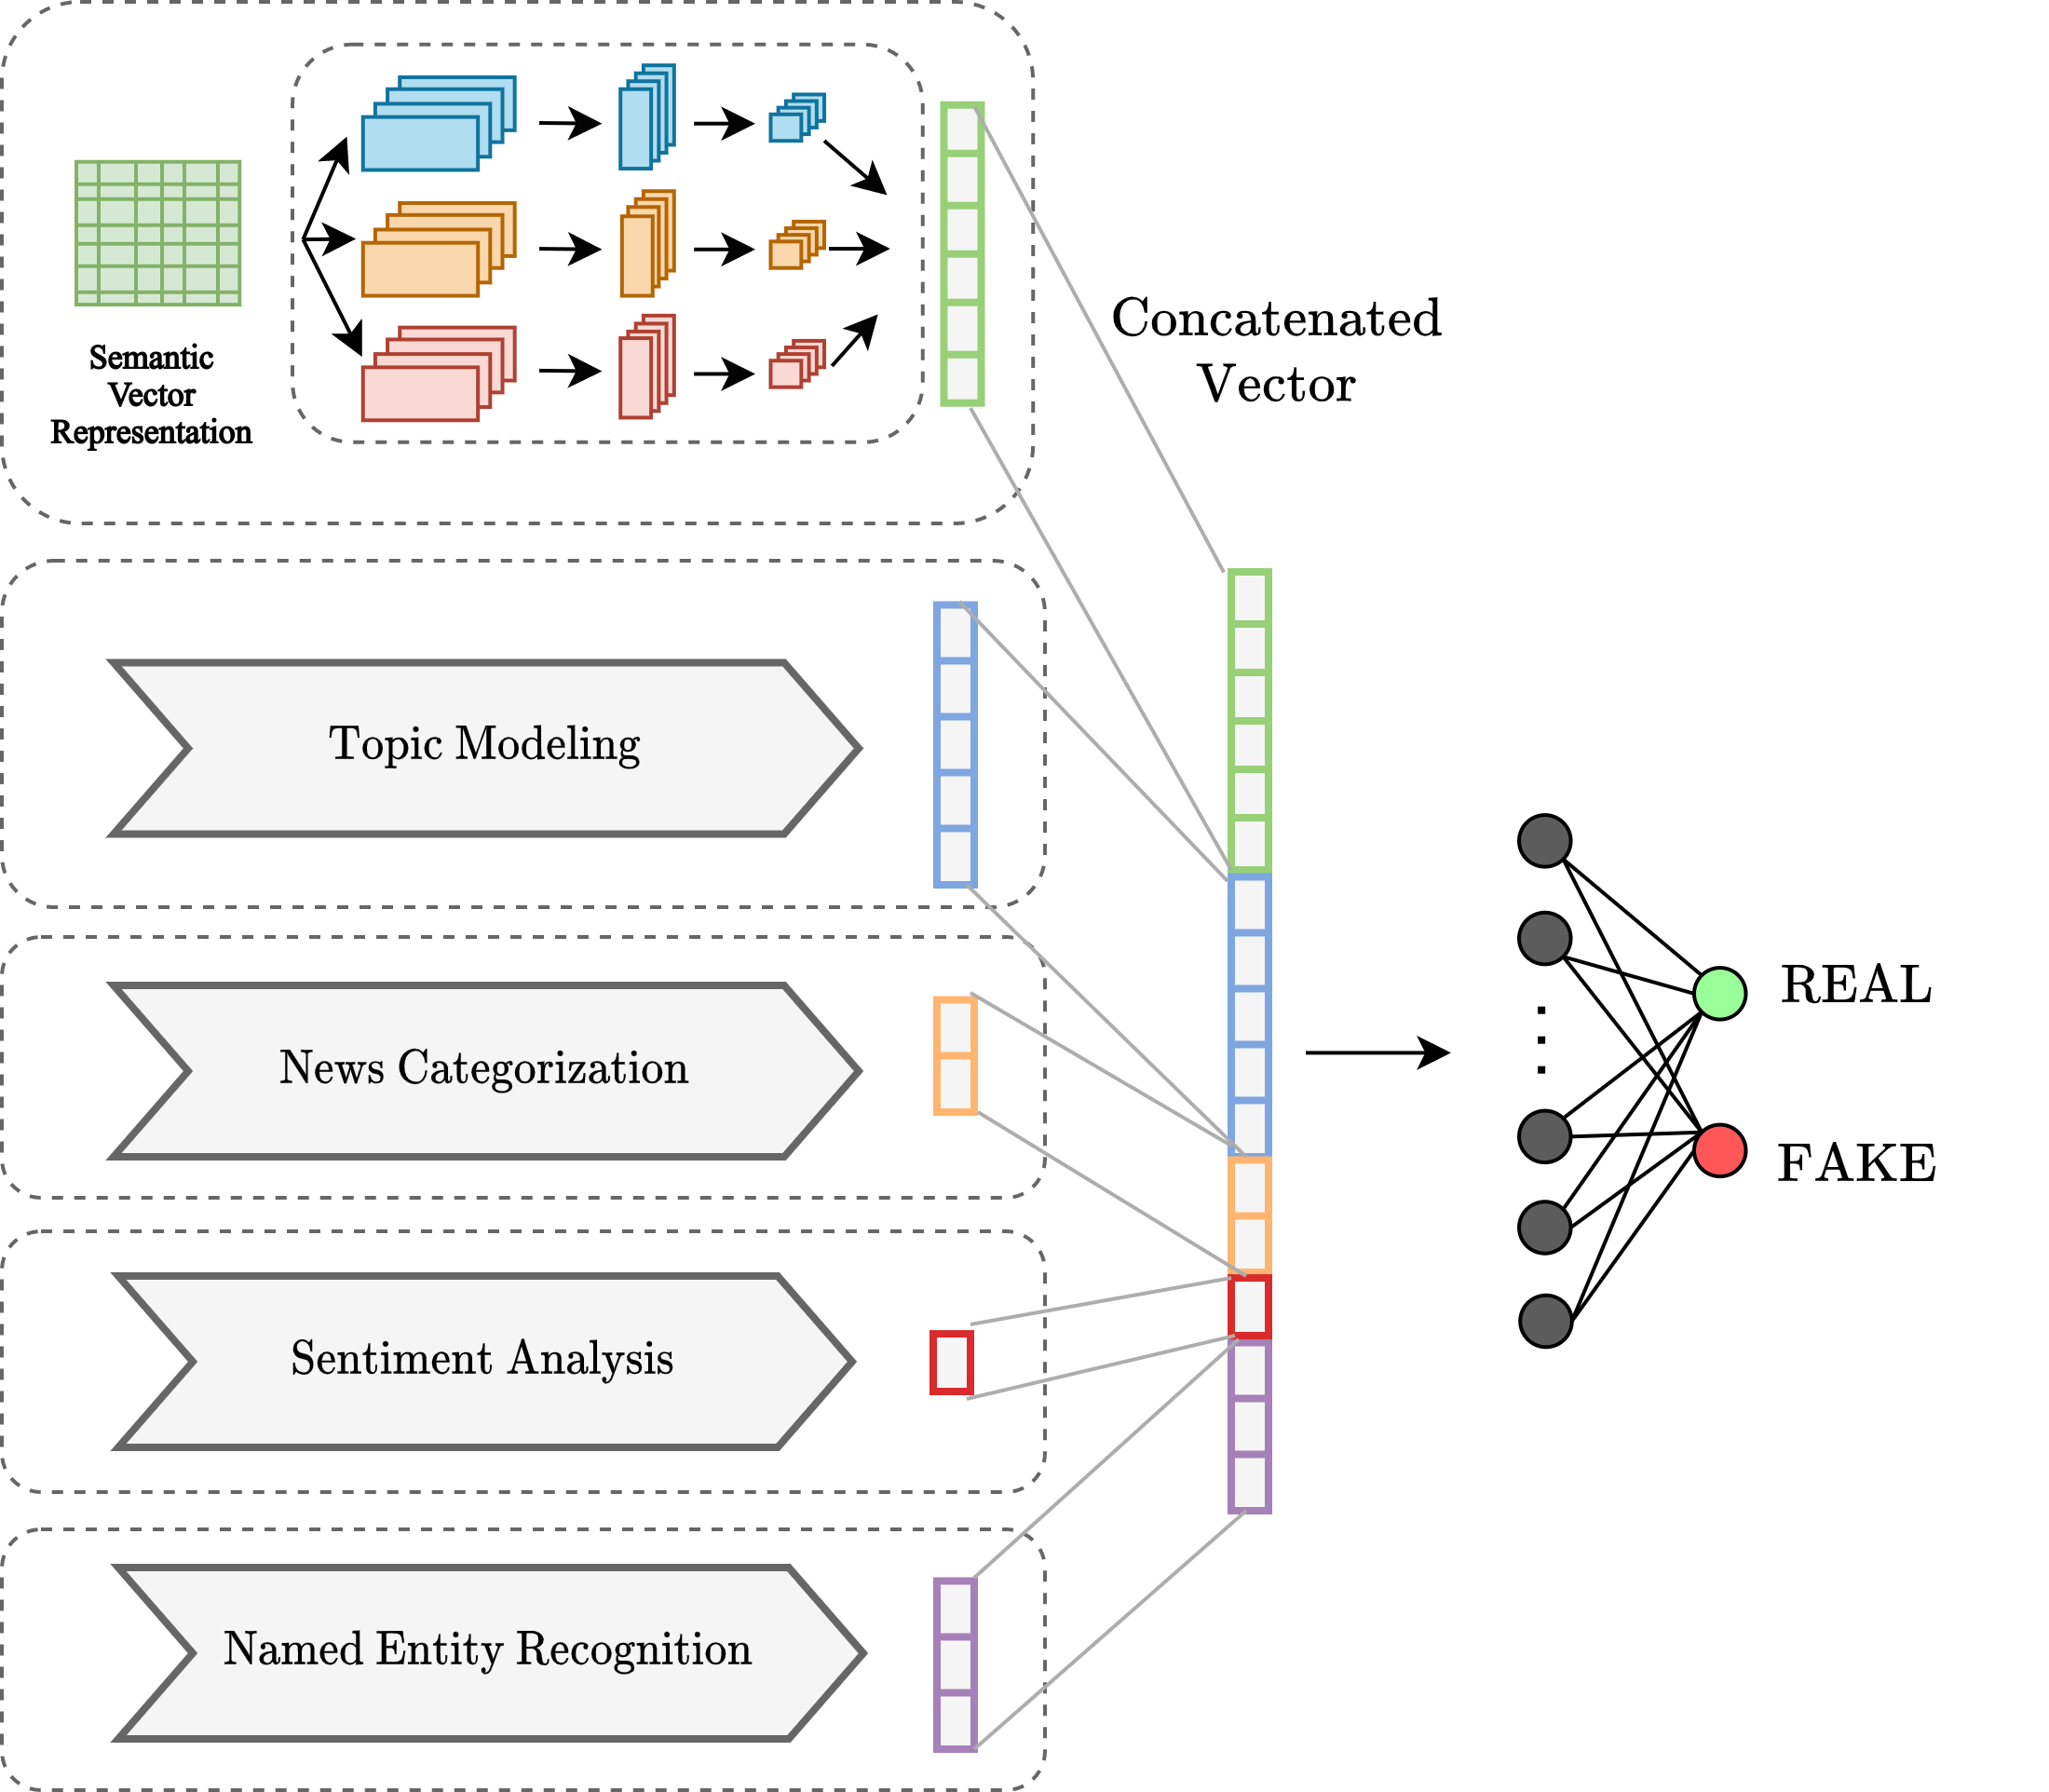
\includegraphics[width=0.75 \textwidth]{all_features}
	\centering
	\caption{شمای کلی مدل ارائه شده برای به‌کار بردن تمام فراداده‌ها و دسته‌بندی اخبار با استفاده از دسته‌بند پیچشی}
	\label{fig.all_features}
\end{figure}

جدول \ref{table.results_meta} نتایج حاصل از استفاده از هریک از فراداده‌های ذکرشده در کنار بازنمایی متنی  در دو دسته‌بند پیچشی و پیشرو را نمایش می‌دهد. دسته‌بند پیچشی ابتدا با استفاده از ماتریس دنباله‌ای مدل پارس‌برت برای متن ورودی، ویژگی‌های سطح بالای مبتنی بر متن را استخراج می‌کند و پس از بهم پیوستن فراداده‌ها به یکدیگر، یک بردار نهایی وارد یک لایه پرسپترون ساده می‌شود تا پیش‌بینی صحت خبر انجام‌شود. در حالت استفاده از دسته‌بند پرسپترون ساده، خروجی تجمعی مدل پارس‌برت استفاده شد و فراداده‌ها به انتها‌ی بردار نماینده متن ورودی اضافه‌ می‌شوند و بردار نهایی به یک لایه چگال وارد می‌شود تا عمل دسته‌بندی انجام‌شود. برای مقایسه راحت‌تر، نتایج حاصل از تشخیص اخبار بدون فراداده که در فصل قبل گزارش شده بود در این جدول تکرار شده‌است.
براساس جدول \ref{table.results_meta}، با استفاده از پردازش‌های متنی توانستیم دقت تشخیص اخبار جعلی را بهبود دهیم. همانطور که انتظار داشتیم دسته‌بند پیچشی توانست عملکرد بهتری را نسبت به مدل شبکه عصبی پرسپترون پیشرو داشته باشد. با توجه به نتایج، ارزشمندترین فراداده که توانست دقت تشخیص مدل ما را بیشتر بهبود دهد، موضوع هر خبر (دسته‌بندی) بود که باعث افزایش \%$1.2$ معیار اف و \%$1.6$ دقت دسته‌بند پیچشی شد. این نتیجه دور از انتظار هم نبود چراکه موضوع هر خبر تاثیر بسیار زیادی در تشخیص اخبار جعلی دارد. همانطور که پیش از این هم اشاره شده، عمده اخبار جعلی در حوزه‌های سیاسی و اجتماعی منتشر می‌شوند. همچنین فراداده‌های مربوط به احساس‌ خبر، بردار موجودیت‌های نام‌د‌ار و موضوع (تخصیص نهان دیریکله) توانستند به طور مجزا دقت نهایی مدل را \%$0.5$، \%$1.35$ و \%$0.3$ افزایش دهند. در نهایت با استفاده از تمامی فراداده‌های استخراج شده از اخبار که با پیوستن به یکدیگر یک بردار ۷۳ بعدی را تشکیل دادند، مدل‌ پارس‌برت-پیچشی ارائه شده را ارزیابی کردیم که باعث افزایش $1.74$ درصدی معیار اف و $1.89$ درصدی دقت شد.

\begin{table}[!t]
	\caption{نتایج تشخیص اخبار جعلی فارسی با استفاده از بازنمایی پارس‌برت و دسته‌بندهای مختلف}
	\label{table.results_meta}
	\begin{center}
		\begin{tabular}{|c|c|c|c|c|c|c|}
			\hline
			بازنمائی & دسته‌بند & فراداده & فراخوانی & صحت & معیار اف & دقت \\
			\hline
			\hline
			\multirow{11}{*}{پارس‌برت} & \multirow{5}{*}{پیچشی}
			& - & $89.13$ & $93.71$ & $91.36$ & $91.64$ \\
			\cline{3-7}
			&  & موجودیت‌های نامدار & $91.16$& $94.28$ & $92.69$ & $92.99$ \\
		\cline{3-7}
			&  & احساس‌ خبر & $91.52$ & $92.57$ & $92.04$ & $92.45$ \\
			\cline{3-7}
			 &  & موضوع  (دسته‌بندی) & $96.87$ & $88.57$ & $92.53$ & $93.26$ \\
			\cline{3-7}
		 &  & موضوع  (تخصیص نهان دیریکله) & $91.42$ & $91.42$  & $91.42$  & $91.91$  \\
			\cline{3-7}
			&  & تمام ویژگی‌ها & $93.64$ & $92.57$ & $93.10$ & $93.53$ \\
			\cline{2-7}
			& \multirow{5}{*}{پرسپترون}
			& - & $92.44$ & $90.85$ & $91.64$ & $92.18$ \\
			\cline{3-7}
			&  &موجودیت‌های نامدار & $93.16$ & $85.71$ & $89.28$ & $90.29$ \\
			\cline{3-7}
			&  &احساس‌ خبر & $83.90$ & $98.28$ & $90.52 $ & $90.29$ \\
			\cline{3-7}
		&  & موضوع  (دسته‌بندی) & $89.13$ & $93.71$ & $91.36$ & $91.64$ \\
			\cline{3-7}
			&  & موضوع  (تخصیص نهان دیریکله)  & $87.89 $ & $95.42$ & $91.50$ & $91.64$ \\
			\hline
		\end{tabular}
	\end{center}
\end{table}